\section{Evaluation}
\label{sec:evaluation}

We have performed experiments both on MicaZ sensors that are part of Motelab, a 38 node
cluster of MicaZ sensors deployed in the Harvard Computer Science building,
as well as performed a variety of simulations on TOSSIM, a TinyOS mote simulator~\cite{hill00}.

\subsection{TOSSIM}
There are several aspects of TOSSIM that make it an unrealistic testbed for
our algorithm which we want the reader to be aware of.
TOSSIM's bit-level radio stack is based on the RFM1000 chip 
which is completely different from the CC2420 in the MicaZ sensors on motelab. 
Thus TOSSIM's radio model is unrealistic for our purposes, 
and furthermore does not currently capture clock skew.  
Additionally, TOSSIM does not model processor time well: 
computation always takes zero time, regardless of the number of instructions, 
and interrupts are instantaneous.
On the the other hand, TOSSIM allows convenient,
direct experimentatation by allowing the user to specify arbitrary topologies, 
and scales to thousands of nodes. Additionally TOSSIM allows addition of user
defined \emph{printfs} to the code which makes debugging a lot simpler
than it is on Motelab.  

In spite of TOSSIM's limitation as a realistic testbed, we choose to 
devote a large part of our evaluation to TOSSIM experiments because it
allows convenient exploration of the parameter space of FICA, our
firefly-based synchronicity scheme. One of our underlying goals is to
throughly explore our synchronicity scheme's parameter space and 
ensure that it is accurate in an ideal testing environment such as TOSSIM.
This will portend well for the effectiveness of our scheme on Motelab, where
testing and debugging is laborious.  It should be noted that attempts to
build clock skew into TOSSIM are currently underway. \\

\subsection{Evaluation Criteria}
\noindent
We focus on two main criteria for evaluating the level of synchronicity achieved:
\begin{enumerate}\addtolength{\itemsep}{-0.5\baselineskip}
\item What is the time taken to achieve synchronicity amongst a group of nodes?
\item How stable is the level of synchronicity achieved?
\end{enumerate}

We define a \emph{period} as the time between firings of two nodes.
For a group of nodes, a period is defined as the time between firings of the
members of that group, where the firings are computed as the
average of the individual mote firings of the group members.
We classify \emph{stability} in terms of consistency of membership 
in a group of sychronized nodes, as well as the consistency of 
the period of the nodes in that group. 
A single group of nodes with a constant number of members, and with a 
regular period, characterizes effective synchronicity. \\

\noindent
{\bf Detecting Groups of Synchronized Nodes} \\
Initial experiments on TOSSIM indicate the possibility
of nodes splitting into separate groups of synchronized entities.
Therefore we have designed our metrics to process data for 
more than one group of synchronized nodes.

In order to detect groups, we have adopted a moving window approach.
In this approach nodes that consistently remain coupled within a certain time period
are grouped together. Given a fixed user-defined window size, the algorithm
finds the best set of motes that fire within that window and 
identifies them as one group. 
This window \emph{moves} over time, and as more firing events are detected, 
group membership is updated.
This is a fairly complex algorithm, and difficult to implement correctly.
Due to space constraints, we do not provide any further details,
and encourage the reader to look at our code repository for a detailed
description of the algorithm.

\subsection{Evaluation Metrics}
We defined the following metrics to evaluate synchronicity in our experiments:

\begin{enumerate}

\item {\bf Group Period}: This measures the length of the period between
which nodes in a group fire.  It is particularly useful to see how the
group period varies with time. Significant variation in a synchronized 
group's period over time will prevent time from advancing uniformly, and
hinders the use of synchronicity for serving as a time synchronization
scheme.

\item {\bf Group Spread}: This measures the extent of variation of 
firing of individual nodes in a group.  This metric captures the precision
of the synchronicity achieved by the nodes.
The standard deviation of the various firing times of the members of group
provides an estimate of how far apart their firing times are.

\item {\bf Time to Achieve Synchronicity}: This measures the 
amount of time it takes for all the nodes in a group to fire 
simultaneously. This metric captures the speed at which synchronicity
is achieved and thus reflects to some extent on the efficiciency of 
our scheme.  Achieving fast synchronicity is crucial for the aforementioned
applicatons in sensor nodes such as power scheduling and coordinated 
data collection.  Whether synchronicity is achieved at all is implicit
in this measure.
This metric is computed by measuring the amount of time taken by 
a certain percentage of motes to form a group and remain in that group
for a certain number of periods.

\item {\bf Group Membership: Nodes entering and exiting}: 
For debugging purposes, it is important to be able to examine 
the membership of individual nodes in a group, and be able to detect whether
group members are being lost, or whether random group members are being
deleted or whether duplicate group members exist.
We use this metric as a means of debugging our 
synchronicity implementation. For a given experiment, this metric
provides a reliable means of determining and verifying 
the quality of group membership.  
\end{enumerate}

\begin{table}
\centering
\caption{Time taken to synchronize (in seconds) for 16 nodes in TOSSIM with different grid topologies, and different values of firing function constants (FFC). The - indicates cases in which synchronization is not achieved.} 
\label{tab:topologyFFC}
%%\subfigure[Table 1: Number of element]
\vspace{2pt}
\begin{tabular}{|r|r|r|r|r|} \hline
Topology                & {\bf FFC=10}  & {\bf FFC=50} & {\bf FFC=100} &   {\bf FFC=200}  \\ \hline
{\bf Grid}              &   90.70    &   73.55     &   84.24        &   266.89      \\ 
{\bf Ring}              &   -        &  123.55     &   77.87        &   194.83      \\ 
{\bf All-To-All}        &   98.43    &   23.44     &   59.35        &   227.05      \\ 
{\bf Line}              &   83.97    &   183.94    &   219.42       &   456.62      \\ \hline
\end{tabular}
\end{table}
\begin{table}
\centering
\caption{Average and Standard Deviation Statistics Per Topology for Table~\ref{tab:topologyFFC}.}
\label{tab:topologyStat}
%%\subfigure[Table 1: Number of element]
\vspace{2pt}
\begin{tabular}{|r|r|r|r|r|} \hline
Topology                & Average    & Standard Deviation \\ \hline
{\bf Grid}              & 128.85     & 92.30 \\ \hline  
{\bf Ring}              & 135.42     & 58.50  \\ \hline  
{\bf All-To-All}        & 102.07     & 88.77  \\ \hline  
{\bf Line}              & 235.99     & 157.87 \\ \hline  
\end{tabular}
\end{table}

\begin{figure}
\begin{center}
\includegraphics[width=1.1\hsize]{./figures/topFFC.pdf}
\end{center}
\caption{{\small {\bf The impact of topology and the magnitude of the firing function constant on the time to synchronize.
The exact values of the time taken to synchronize are listed in~\ref{tab:topologyFFC}.}}} 
\label{fig:topFFC}
\end{figure}

\begin{figure}[t]
\begin{center}
\includegraphics[width=1.0\hsize]{./figures/5-Jan-2005-1-RING-NODES-16-50CONSTANT-GROUP-PERIOD.pdf}
\end{center}
\caption{{\small {\bf Group period for 16 node ring topology with firing function constant 50.}}} 
%{\em This figure shows...}}}
\label{fig:rgp}
\end{figure}

\begin{figure}[t]
\begin{center}
\includegraphics[width=1.0\hsize]{./figures/5-Jan-2005-1-RING-NODES-16-50CONSTANT-GROUP-SPREAD.pdf}
\end{center}
\caption{{\small {\bf Group spread for 16 node ring topology with firing function constant 50.}}}
%{\em This figure shows...}}}
\label{fig:rgs}
\end{figure}

\begin{figure}[t]
\begin{center}
\includegraphics[width=1.0\hsize]{./figures/5-Jan-2005-1-LINE-NODES-16-50CONSTANT-GROUP-PERIOD.pdf}
\end{center}
\caption{{\small {\bf Group period for 16 node line topology with firing function constant 50.} }}
%{\em This figure shows...}}}
\label{fig:lgp}
\end{figure}

\begin{figure}[t]
\begin{center}
\includegraphics[width=1.0\hsize]{./figures/5-Jan-2005-1-LINE-NODES-16-50CONSTANT-GROUP-SPREAD.pdf}
\end{center}
\caption{{\small {\bf Group spread for 16 node line topology with firing function constant 50.} }}
%{\em This figure shows...}}}
\label{fig:lgs}
\end{figure}

\begin{figure}[t]
\begin{center}
\includegraphics[width=1.0\hsize]{./figures/5-Jan-2005-1-GRID-NODES-16-50CONSTANT-GROUP-PERIOD.pdf}
\end{center}
\caption{{\small {\bf Group period for 16 node 4by4 regular grid topology with firing function constant 50.} }}
%{\em This figure shows...}}}
\label{fig:ggp}
\end{figure}


\begin{figure}[t]
\begin{center}
\includegraphics[width=1.0\hsize]{./figures/5-Jan-2005-1-GRID-NODES-16-50CONSTANT-GROUP-SPREAD.pdf}
\end{center}
\caption{{\small {\bf Group spread for 16 node 4by4 regular grid topology with firing function constant 50.} }}
%{\em This figure shows...}}}
\label{fig:ggs}
\end{figure}


\begin{figure}[t]
\begin{center}
\includegraphics[width=1.0\hsize]{./figures/5-Jan-2005-1-ALL-NODES-16-50CONSTANT-GROUP-PERIOD.pdf}
\end{center}
\caption{{\small {\bf Group period for 16 node all-to-all topology with firing function constant 50.} }}
%{\em This figure shows...}}}
\label{fig:agp}
\end{figure}

\begin{figure}[t]
\begin{center}
\includegraphics[width=1.0\hsize]{./figures/5-Jan-2005-1-ALL-NODES-16-50CONSTANT-GROUP-SPREAD.pdf}
\end{center}
\caption{{\small {\bf Group spread for 16 node all-to-all topology with firing function constant 50.} }}
%{\em This figure shows...}}}
\label{fig:ags}
\end{figure}




\subsection{TOSSIM Experiments}
A number of simulation experiments have been performed on TOSSIM to evaluate
the impact of different parameters of the model on the accuracy and
quality of synchronicity achieved amongst the nodes.  We explore the impact
of parameters such as the firing function constant (a constant value that
is equal to $\frac{1}{\epsilon}$, where $\epsilon$ is the firing function
related quantity discussed in sections~\ref{sec:fireflyModel} and ~\ref{sec:firingFunc}), 
and the number of nodes on the quality of synchronicity achieved as 
measured by group spread, group period and time taken to synchronize.

Fig.~\ref{fig:topFFC} shows the values of time to synchronize for 16 nodes with different
topologies and firing function constants.  It is obvious that a higher firing function
constant does not imply consistently lower time to synchronization.  Overall nodes in the
line topology takes the longest time to synchronize except when the firing function constant
is 10. 
Nodes in the all-to-all topology generally take less time to synchronize than the other
topologies. This is not surprising since all-to-all is the best conceivable topology.
Tables~\ref{tab:topologyFFC}-~\ref{tab:topologyStat} show numerical values of the
time taken to synchronize (in seconds) for different topologies and firing function
constant values. The standard deviations give an idea of the large extent to
which the firing function constant can influence the time taken to achieve synchronicity.
In Table~\ref{tab:topologyStat} the line topology has the highest standard deviation,
and indicates that this topology is particularly vulnerable to changes in the firing function
constant.

Fig.~\ref{fig:rgp}-~\ref{fig:ags} show the group period and group spread of 16 nodes
with four different topologies: line, 4by4 regular grid, ring and all-to-all.
It is reassuring to see that for all node topologies, the group period stabalizes
at 1 after a given time period.  The group period of the line topology takes the
longest time to stabalize (190 seconds), while the group period of the all-to-all topology 
takes the shortest amount of time to stabalize (less than 30 seconds). Similarly
the group spread of the all-to-all topology has the least amount of variation,
and the group spread of the line topology has the most amount of variation.
The reason for this is quite intuitive. In the line topology, nodes towards the ends
of the lines have difficulty detecting all the fires. On the other hand, nodes in the
all-to-all connected topology are well connected to all their neighbors and
can efficiently respond to detected fires.


%% Geoff's graphs here

\begin{figure}[t]
\begin{center}
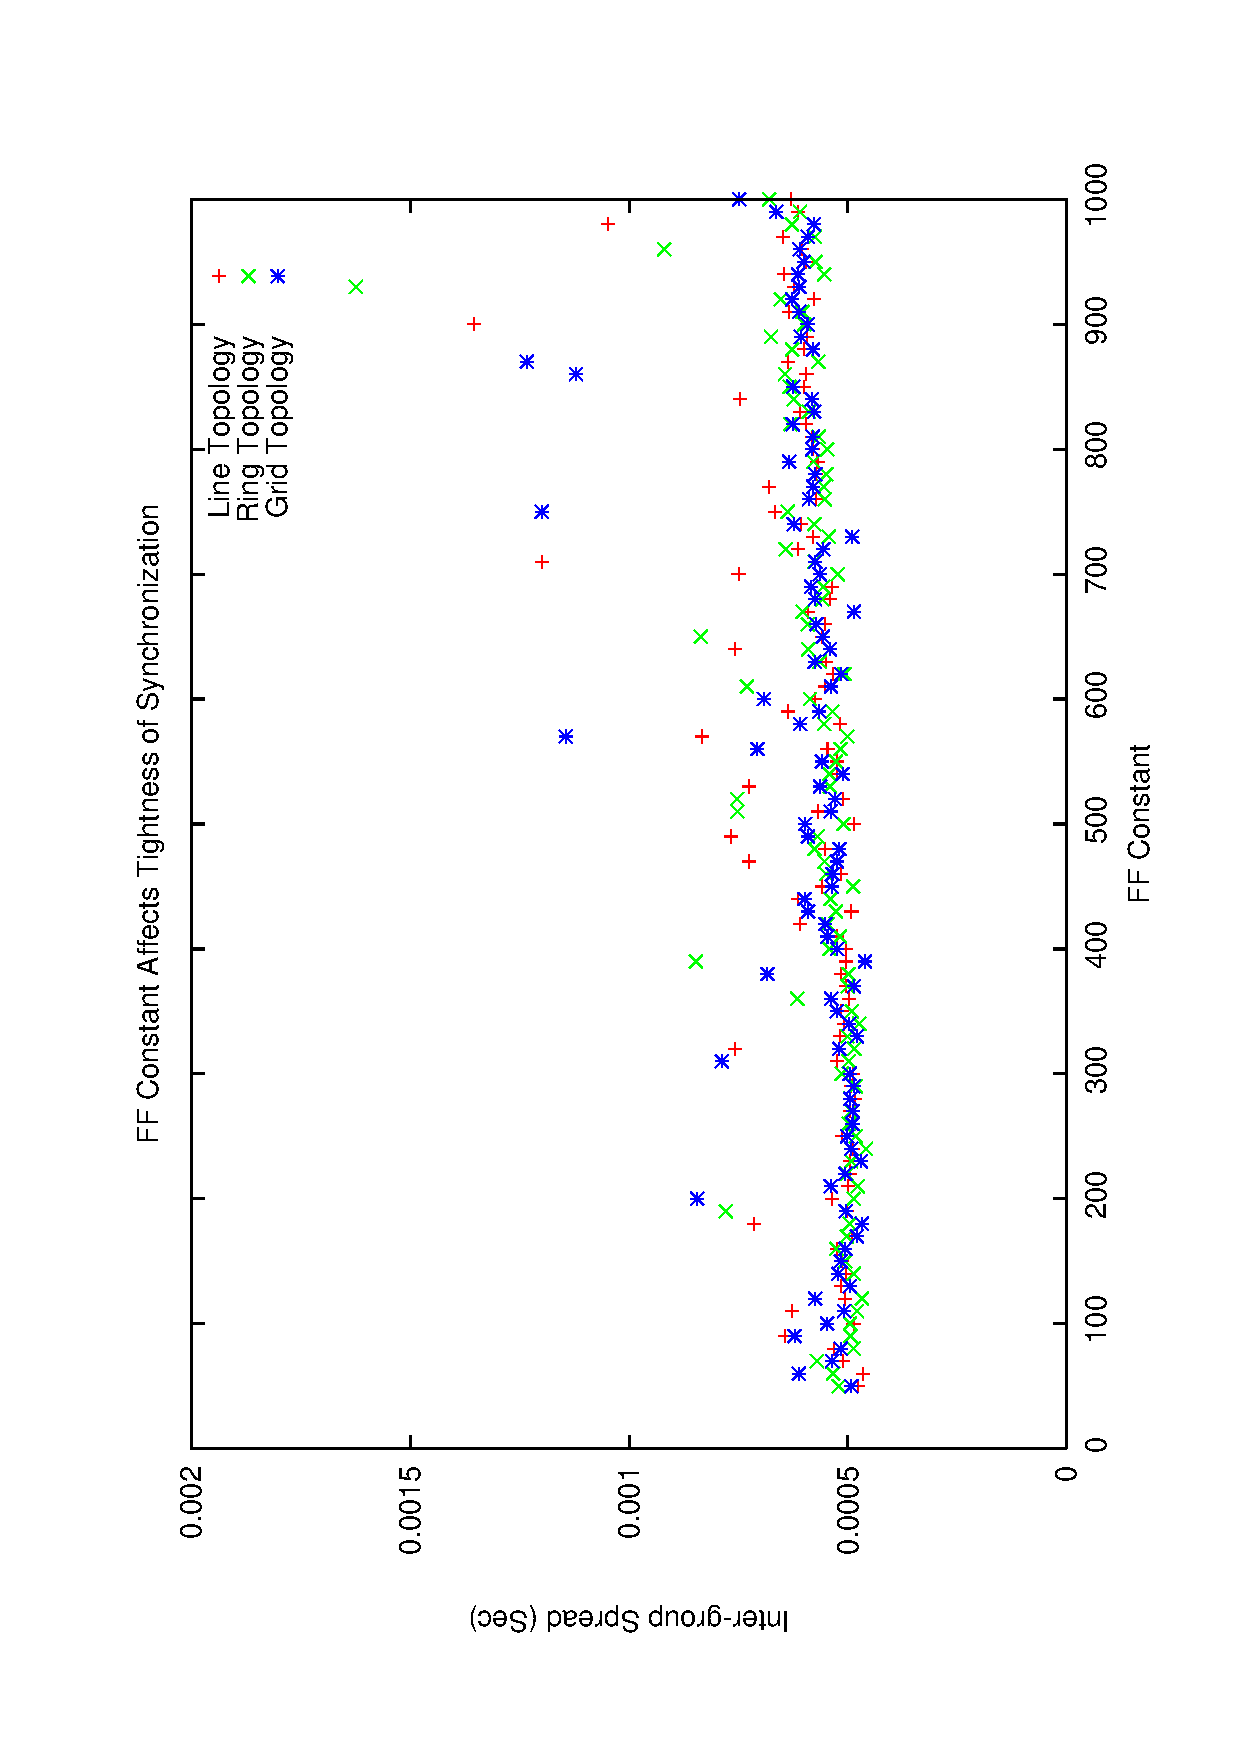
\includegraphics[width=1.0\hsize]{./figures/16-NOADD-LINERINGGRIDALLALL-SPREAD.pdf}
\end{center}
\caption{{\small {\bf The impact of the firing function constant on the group spread for three different node topologies}}}
\label{fig:lgp}
\end{figure}

\begin{figure}[t]
\begin{center}
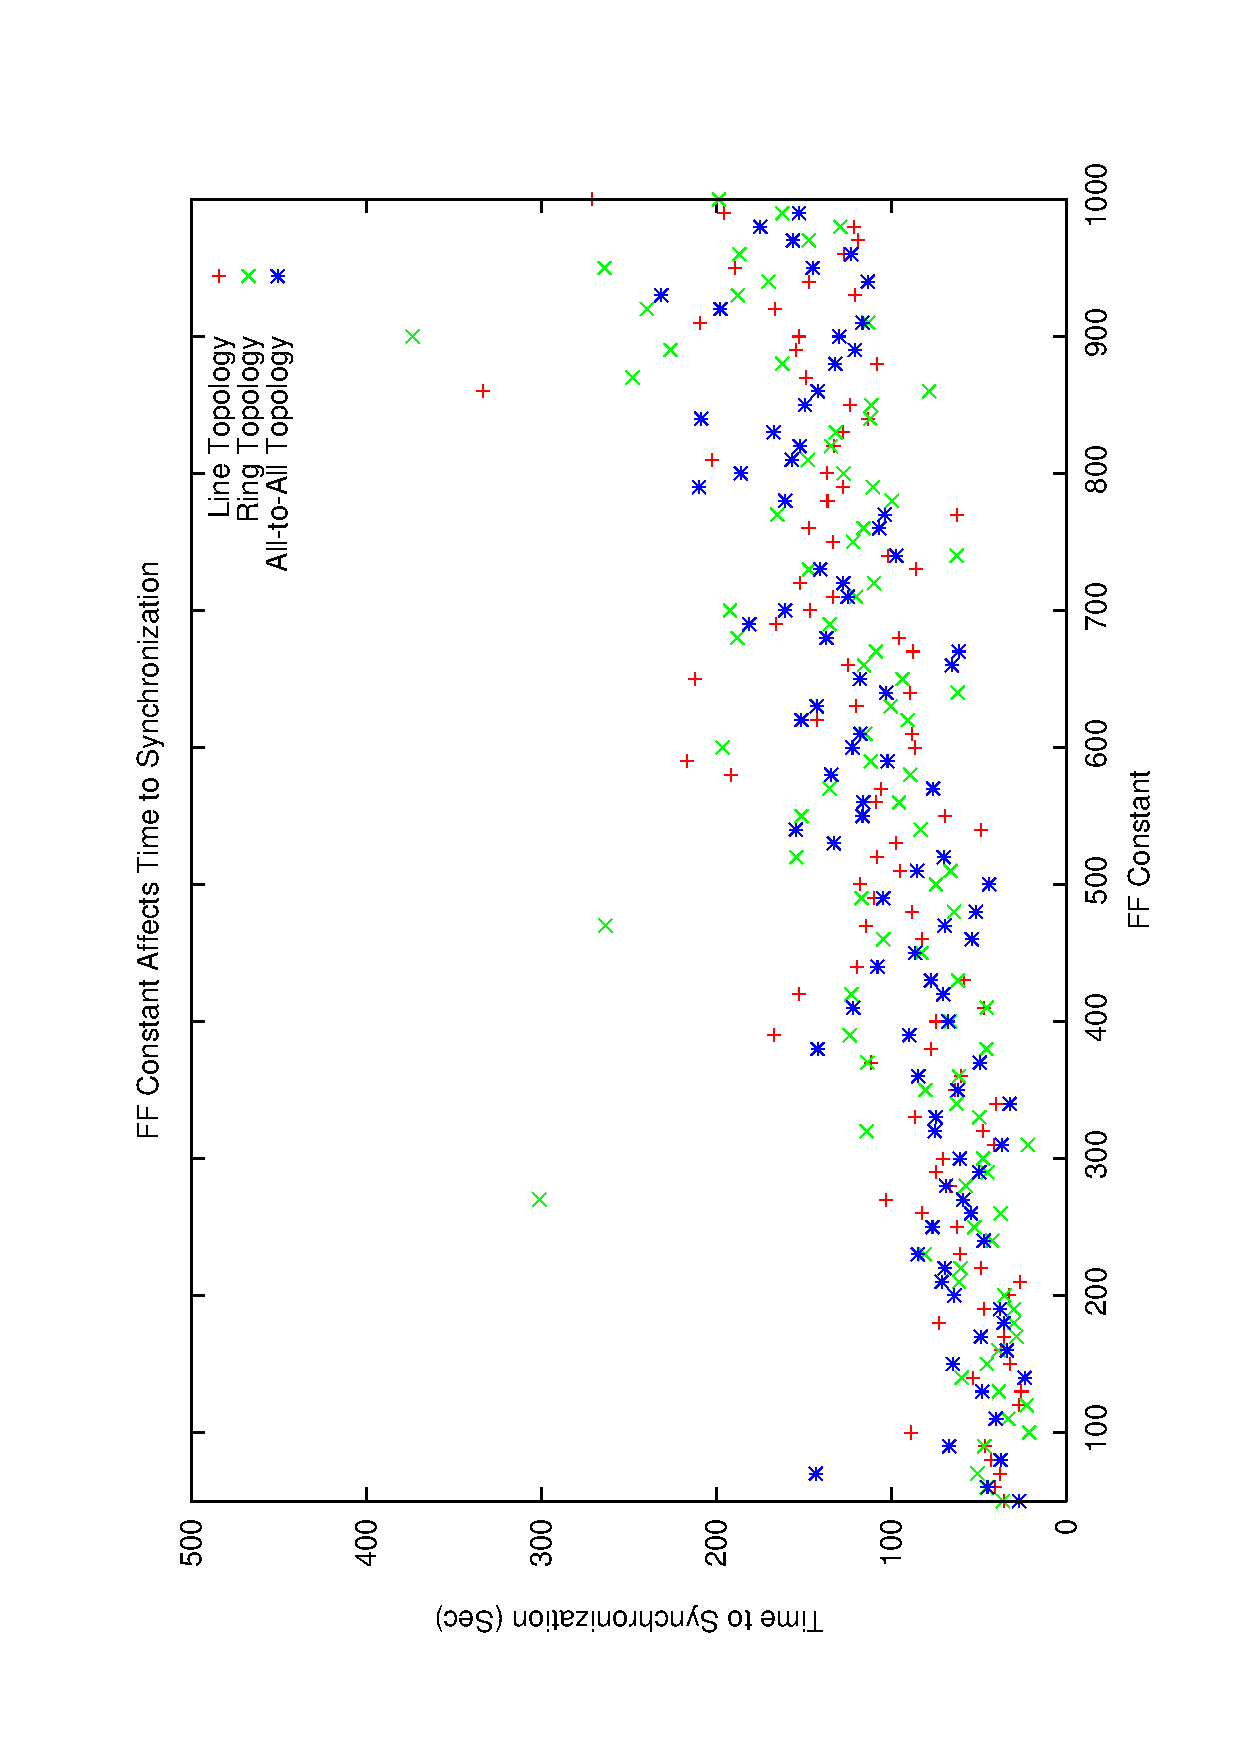
\includegraphics[width=1.0\hsize]{./figures/16-NOADD-LINERINGALLTOALL.pdf}
\end{center}
\caption{{\small {\bf The impact of the firing function constant on the time taken to synchronize for three different node topologies.}}}
\label{fig:lgp}
\end{figure}

\begin{figure}[t]
\begin{center}
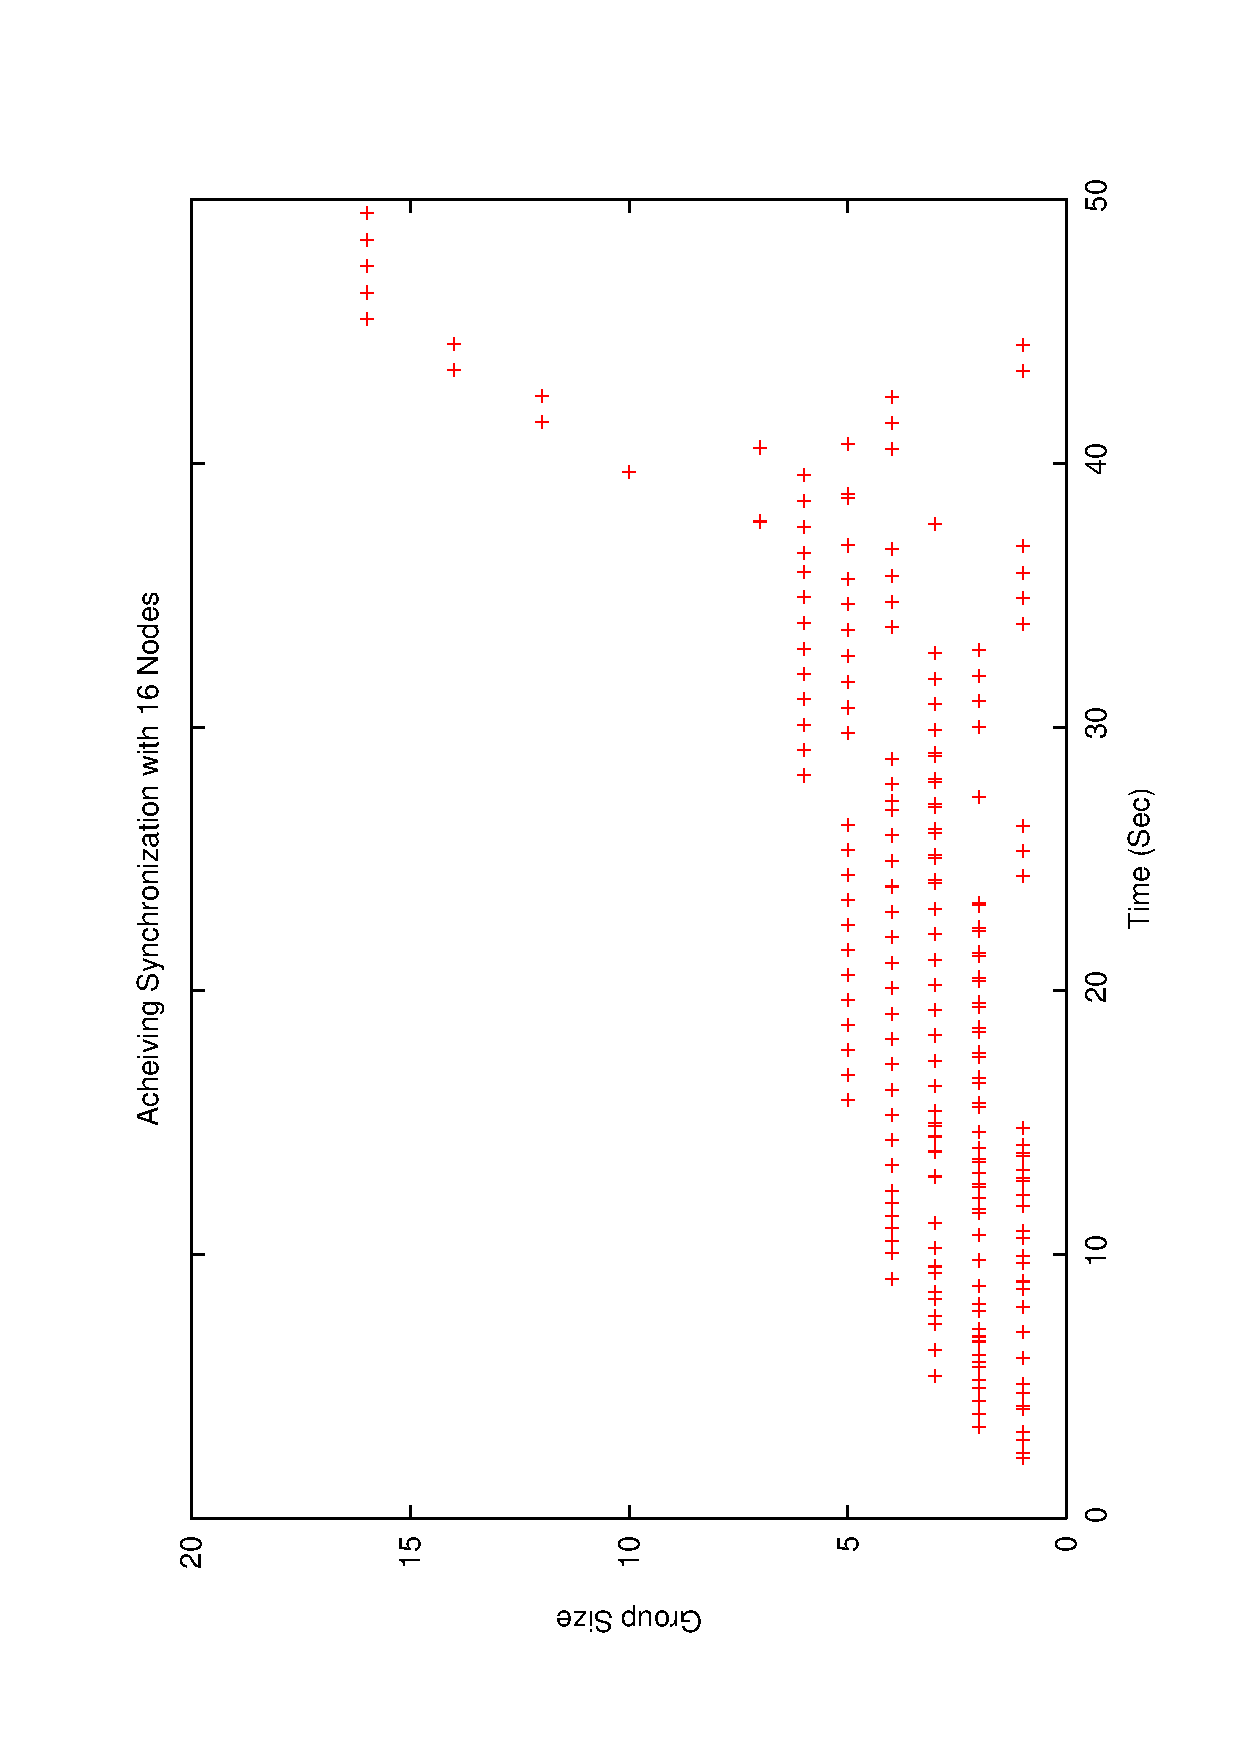
\includegraphics[width=1.0\hsize]{./figures/11-Jan-2005-1-16MOTES-150CONSTANT-RING-EVENT-ALL-GROUPS.pdf}
\end{center}
\caption{{\small {\bf The size of a group over time.}}}
\label{fig:lgp}
\end{figure}


